\section{Identificação do problema}
\begin{frame}{Proposta}
	\begin{itemize}
		\item Definição / exemplo 1
		\item Definição / exemplo 2
		\item Definição / exemplo 3
	\end{itemize}
\end{frame}

\section{Conscientização do problema}
	\begin{frame}{Relações causais sob análise}
		\centering
		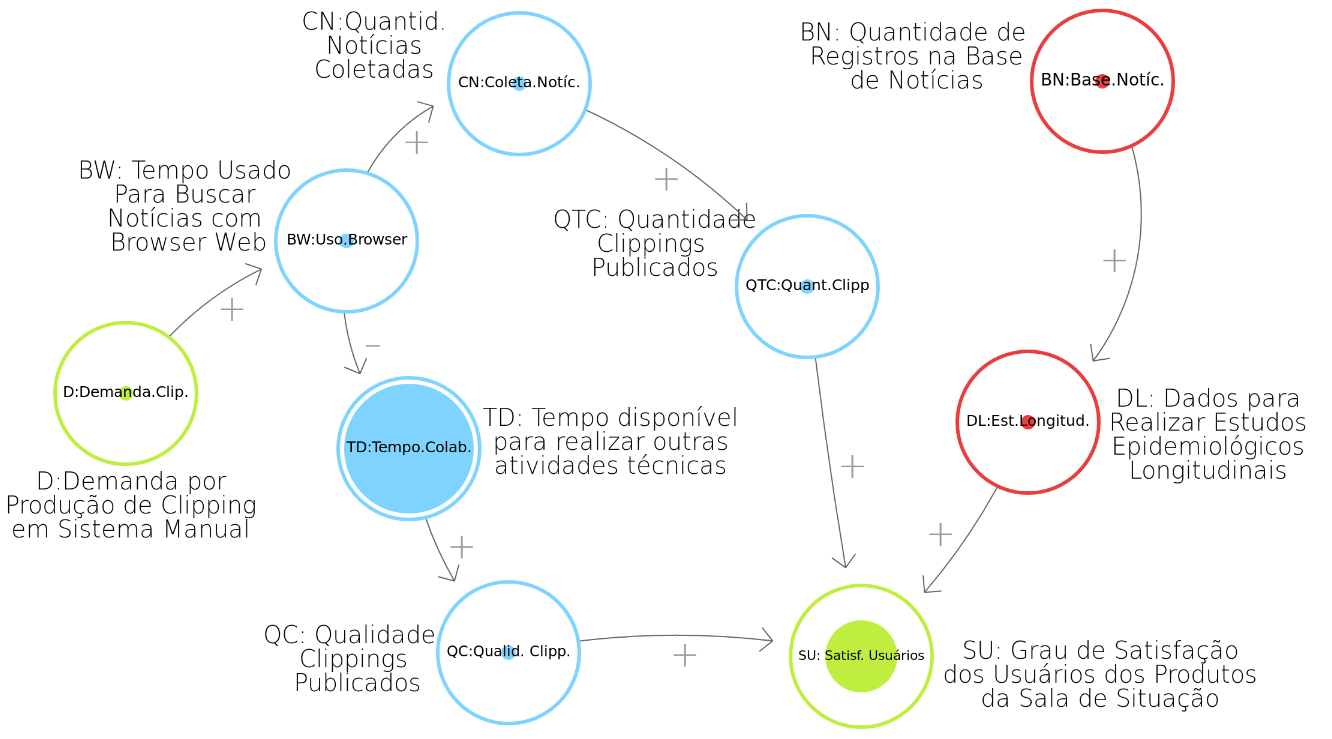
\includegraphics[width=0.8\textwidth]{ProducaoClippingManual.png}
	\end{frame}

%\section{Revisão da literatura}

\section{Identificação dos artefatos}
\begin{frame}{Artefatos Identificados}
	\begin{itemize}
		\item Definição / exemplo 1
		\item Definição / exemplo 2
		\item Definição / exemplo 3
	\end{itemize}
\end{frame}

\section{Proposição de artefatos}
\begin{frame}{Artefatos Propostos}
	\begin{itemize}
		\item Proposição / exemplo 1
		\item Proposição / exemplo 2
		\item Proposição / exemplo 3
	\end{itemize}
\end{frame}

\section{Projeto do artefato selecionado}
\begin{frame}{Projeto dos Artefatos}
	\begin{itemize}
		\item Diagrama / exemplo 1
		\item Diagrama / exemplo 2
		\item Diagrama / exemplo 3
	\end{itemize}
\end{frame}

\section{Desenvolvimento do artefato}
\begin{frame}{Atributos Técnicos dos Artefatos Desenvolvidos}
	\begin{itemize}
		\item Atributo / exemplo 1
		\item Atributo / exemplo 2
		\item Atributo / exemplo 3
	\end{itemize}
\end{frame}

\section{Implementação do artefato}
\begin{frame}{Como ocorreu a implementação?}
	\begin{itemize}
		\item Atributo / exemplo 1
		\item Atributo / exemplo 2
		\item Atributo / exemplo 3
	\end{itemize}
\end{frame}

\section{Avaliação do artefato}
\begin{frame}{Resultados das Avaliações}
	\begin{itemize}
		\item Resultado / exemplo 1
		\item Resultado / exemplo 2
		\item Resultado / exemplo 3
	\end{itemize}
\end{frame}

\section{Explicitação das aprendizagens}
\begin{frame}{O que o grupo aprendeu?}
	\begin{itemize}
		\item Aprendizagem / exemplo 1
		\item Aprendizagem / exemplo 2
		\item Aprendizagem / exemplo 3
	\end{itemize}
\end{frame}

\section{Conclusões}
\begin{frame}{Conclusões sobre a Realização do Projeto}
	\begin{itemize}
		\item Objetivos Alcançados? / exemplo 1
		\item Objetivos Alcançados? / exemplo 2
		\item Objetivos Alcançados? / exemplo 3
	\end{itemize}
\end{frame}

\section{Generalização para uma classe de problemas}
\begin{frame}{Generalização }
	\begin{itemize}
		\item Generalização / exemplo 1
		\item Generalização / exemplo 2
		\item Generalização / exemplo 3
	\end{itemize}
\end{frame}



